\documentclass[a4paper]{article}

%%% packages %%%%%%%%%%%%%%%%%%%%%%%%%%%%%%%%%%%%%%%%%%%%%%%%%%%%%%%%%%%%%%%%%
\usepackage{graphicx}
\usepackage[utf8]{inputenc}
%\usepackage[T1]{fontenc}
\usepackage[ngerman]{babel}
\usepackage{subcaption}
\usepackage{amsmath,amssymb}
\usepackage{alltt}
\usepackage{natbib} % please use \citep and \citet instead of \cite
\usepackage{tikz}
\usetikzlibrary{positioning,automata}
\usetikzlibrary{shapes.geometric}
\usetikzlibrary{shapes.arrows}
\usepackage{array}
\usepackage{hyperref}
\usepackage{xcolor}
\usepackage{listings}
\usepackage[export]{adjustbox}
\definecolor{dark-red}{rgb}{0.4,0.15,0.15}
\definecolor{dark-blue}{rgb}{0.15,0.15,0.8}
\definecolor{medium-blue}{rgb}{0,0,0.5}
\hypersetup{
	colorlinks, linkcolor={dark-red},
	citecolor={dark-blue}, urlcolor={medium-blue}
}

\graphicspath{{./figs/}}
\DeclareGraphicsExtensions{.pdf}

\setlength{\parindent}{0mm}

\usepackage{fancyhdr}

%%% %%%%%%%%%%%%%%%%%%%%%%%%%%%%%%%%%%%%%%%%%%%%%%%%%%%%%%%%%%%%%%%%%%%%%%%%%

\makeatletter
\newcommand{\seminar}{Ambient Computing (SS 2019)}
\title{\textbf{Ambient Computing:\\ Zusammenfassung}}\let\Title\@title
\newcommand{\sTitle}{Drahtlose Sensornetze}
\newcommand{\AuthorName}{Alexander Osiik}
\author{\AuthorName\\
	\href{mailto:alexander.osiik@student.uni-luebeck.de}{alexander.osiik@student.uni-luebeck.de}\\
	\small \seminar\\
	%    \small Service Robotics Group\\
	\small Institute of Computer Engineering, University of L\"ubeck\\
}\let\Author\@author
\makeatother

\pagestyle{fancy}
\renewcommand{\footrulewidth}{0.4pt}
\lfoot{\seminar}
\cfoot{}
\rfoot{\thepage}
\lhead{\AuthorName}
\rhead{\sTitle}

%%% %%%%%%%%%%%%%%%%%%%%%%%%%%%%%%%%%%%%%%%%%%%%%%%%%%%%%%%%%%%%%%%%%%%%%%%%%

\begin{document}
	\maketitle	
\section{Einführung}
\subsection{Was ist Ambeint Computing?}
Bei Ambient Computing handelt es sich um \textbf{vernetzte}, in einer \textbf{Umgebung} \textbf{eingebetteten} \textbf{Systeme}, die \textbf{allgegenwärtig}, und für den Nutzer \textbf{unsichtbar}, die den Nutzer abhängig vom \textbf{Kontext} der Umgebung assistieren. \\

Das Ambiente ist dabei
\begin{itemize}
	\item \textbf{physikalisch},
	\item \textbf{visuell}, 
	\item \textbf{sensorisch}, 
	\item \textbf{virtuell}
\end{itemize}
erfassbar und für jeden anders!\\

Hier liegen bereits die erste Schwierigkeiten vor, da es keine klare übergreifende Definition für Ambiente, Umgebung, Kontext etc. gibt.
\begin{itemize}
	\item \textbf{Umgebung/Raum} wird durch seine physikalischen Eigenschaften, Subjekte und Orte definiert.\\
	Hierbei kann der Raum über einen \textbf{intendierten Nutzungskontext} verfügen (zB Küche, Seminarraum, Krankenhaus). Die Computer müssen also in die Lage versetzt werden, das Ambiente und den \textbf{Sinn des Raumes} zu erkennen.
	\item Der \textbf{Nutzungskontext} ist dabei das, was für den Nutzer und die Anwendung relevant ist. Eine klare Definition gibt es nicht, jedoch gehören das \textbf{Subjekt}, der \textbf{Ort}, die \textbf{Dinge}, die \textbf{Anwendungen} und die \textbf{Intentionen} dazu.
\end{itemize} 
\subsection{Beispiele}
\begin{itemize}
	\item[\textbf{Ambient Light:}] In der Computergrafik ist es die natürliche Beleuchtung. Das Produkt sind Lichtspiele hinter einem TV-Gerät, die das Fernsehbild über den TV hinaus vergrößern.  
	\item[\textbf{Ambient Music:}] Musik für Ambiente, in dem Musik nicht Fokus liegt, zB am Flughafen. Ziel sind induzierte Beruhigung oder Kaufwille.
	\item[\textbf{Ambient Media:}] Die Umgebung wird als Werbefläche missbraucht.. äh.. benutzt. Es wird einem ein Produkt untergejubelt allein dadurch, dass man es sieht. Man wird also gezwungen, Werbung zu schauen.
	\item[\textbf{Ambient Comp.:}] Angebrachte \textbf{Sensorik}, die gewisse Metadaten misst und erfasst, und die zugehörige \textbf{Aktorik}. die dann den \textbf{Kontext} modifiziert. 
\end{itemize}
Optimale Sensorik und Aktorik wären beispielsweise Nanotechnologie oder sich selbst verändernde Materialien oder Objekte. Sich selbst anpassende Tische, Stühle, Boards etc. Bei Ambient Computing soll dabei der Fokus auf die vereinfachte Arbeit mit \textbf{Informationen} liegen, und nicht mit Materialien.
\subsection{Evolution von Computing}
Mittlerweile sind wir in der Lage, den Computer ins Ambiente zu tragen, auch wenn das Ambiente dafür nicht vorgesehen ist. Um den Computer nun an jeden Ort des Universums anpassbar zu machen, brauchen wir eine Ontologie für das Universum, was unmöglich zu bewerkstelligen ist.
Man will eigentlich nichts mehr bei sich tragen müssen, sondern beim Betreten einer Umgebung alles bereits da haben.  \\

\textbf{Will man ein Rechner sein oder in einem Rechner leben?}\\

``\textit{The old computing is about what computers can do - the new computing is about what people can do}'' - \textbf{Ben Shneiderman}\\

Der heutige Zweck dieses wissenschaftlichen Feldes ist, Alltagsgegenstände smart zu machen, um das menschliche Lebensumfeld zu verbessern und mit ambienten Rechnern zu optimieren. Beispiele für heutige Computer sind
\begin{itemize}
	\item Smart Dust
	\item Smart Mirrors
	\item Smarte Wasserhähne
	\item Smart Bite uvw.
\end{itemize}
Menschen wollen ihr Umfeld verbessern, um das Interesse zu \textbf{delegieren} und \textbf{Ressourcen} zu sparen. Es obliegt also die Wahl zwischen \textbf{Delegation} und \textbf{Domain Expertise}.\\

\subsection{Wie weit soll man gehen?}
Smarte Systeme müssen nicht nur die eigenen Wünsche, sondern auch dir Wünsche anderer mitbetrachten. Man benötigt also ethische Regeln für Computer (Autonomes Fahren), bevor die Technologie dei Menschheit ``versklavt'' (2001: A Space Odyssey).\\

Smarte Gadgets kommen meist in Form von IoT-Geräten. Wenn man jedoch jeden Alltagsgegenstand smart macht, hat man am Ende 10.000 Gegenstände die man administrieren muss (Softwareupdate, Akku, Steckplätze, Bedienung etc). Hinzu kommt, dass die \textbf{Kommunikation} zwischen Mensch und Aktor in der Regel nicht trivial ist; man benötigt also neue \textbf{Interaktionmechanismen}.\\

 Die Technik weiß dabei meist mehr, als der Nutzer, und dieses Wissen muss dm Nutzer mitgeteilt werden - Diskussion mit Technik?

\newpage
\section{Ambiente in der Computergeschichte}
Der Abakus war wahrscheinlich das erste Rechensystem der Menschengeschichte, welcher bis ins 17. Jahrhundert der State-of-the-Art war.\\
Ab dem 17.Jhd entwickelte man mechanische Computer und das \textbf{binäre Rechensystem}(1679), bis dann 1960 die ersten \textbf{Transistor Computer} auf den Markt kamen.
\subsection{Was ist ein idealer PC?}
Ein für den Nutzer idealer PC wäre einer bei dem alle Wünsche und Anforderungen des Nutzers ab Werk konfiguriert sind. Dafür muss der Hersteller sich in jeden Nutzer hineinversetzen können, was praktisch gesehen nur durch einen unerwünschten Eingriff in die Privatsphäre bedeuten würde. Schließlich möchten die wenigsten Nutzer sich selbst verkaufen.

\subsection{Influencer von Ambient Computing}
\begin{itemize}
	\item \textbf{Vannevar Bush (1890-1974)} hatte die Idee von einer theoretischen Maschine namens \textbf{memex}, mit der Dokumente gespeichert und aufgerufen werden können. Diese wurden mit Bildern assoziiert. \\
	$\rightarrow$ Vision vom Internet
	\item \textbf{MyLifeBits Projekt (seit 2001)} ist ein Projekt von Microsoft und stellt eine persönliche Datenbank für Alles dar.
	\item \textbf{J.C.R Licklider (1915-1990)} hatte 1960 damit begonnen, Computerschnittstellen zu entwickeln. Seine Ideen waren Grundbaustein für \textbf{point-and-click} Schnittstellen, digitale \textbf{Bibliotheken}, \textbf{eCommerce} etc.
	\item \textbf{Douglas Englebart (1925-2013)} wollte die Ideen von \textbf{Bush} aufgreifen und das menschliche Intellekt mit Computern erweitern. Er war der Entwickler der \textbf{Maus}, \textbf{Hypertext}, \textbf{Objektadressierung} und shared-screen-\textbf{Kollaboration}.
	\item \textbf{Myron Krueger (1945-)} sprach 1977 von den \textbf{Responsive Environments}, in denen den Gliedmaßen des Nutzers neue Bedeutung gegeben worden ist. Er war maßgeblich an der Forschung der \textbf{Mensch-Computer Interaktion} beteiligt. Der Nutzer wart \textbf{Komponist} der intelligenten Systemumgebung. 
\end{itemize}

\subsection{Computer - Historische Entwicklung}
Die erste Ära der Computer begann 1960 mit dem ``Transistor Computer''. Dabei war das damalige Paradigma, dass \textbf{viele} Menschen \textbf{eine} teure Ressource teilten, die zudem nur beschränkten Zugriff hatte.\\

In den 70er-Jahren kamen dann die ersten ``Mikroprozessor Computer'' auf den Markt; die zweite Ära des Computer begann. Das Paradigma: \textbf{Jeder} Mensch hat seinen \textbf{eigenen} persönlichen Computer, den er ohne Zugriffseinschränkung nutzen konnte.\\

Im Jahr 1981 bahnte sich ein neuer Paradigmenwechsel an. Mit dem ``Osborne 1'' wurde ein\textbf{ mobiler Compute}r auf den Markt gebracht.\\
Bei \textbf{Mobilität} unterscheidet man in drei Kategorien:
\begin{itemize}
	\item \textbf{Device Mobility:} Man kann das Gerät an einen anderen Ort bewegen
	\item \textbf{User Mobility:} Der Nutzer kann problemlos das Gerät wechseln
	\item \textbf{Session Mobility:} Die Sitzungen werden während der Bewegung gespeichert/weitergeführt 
\end{itemize}

\newpage
\section{Ubiquitous Computing}
``\textit{Ubiquitous Computing enhances computer use by making computers available throughout the physical environment, while making them \underline{effectively invisible} to the user}'' - \textbf{Mark Weiser (1952-1999)}\\

Ubiquitous Computing stellt die neue Äre der Computernutzung nach ``Personal Computing'' (2. Ära) dar. Die Idee war, überall Computer zu haben, die jedoch für den Menschen \textbf{unsichtbar} sind. Unsichtbar in dem Sinne, dass der Mensch nicht merkt, dass er ein Computer benutzt. Computer werden so alltäglich, dass sie nicht mehr wahrgenommen werden.\\

Die besten Technologien sind demnach die, die in der Umgebung verschwinden, und die so in das tägliche Leben integriert sind, sodass das das neue Leben ist. Die Nutzung des Computers soll dabei ``wie bei Schluck Wasser nehmen'' sein: Man soll über den Prozess nachdenken, nicht über den PC.

\subsection{Ubiquitousness / Allgegenwärtigkeit}
Das beste Beispiel für Allgegenwärtigkeit ist dabei der Elektromotor.\\
 Früher waren diese rar und wertvoll, wurden nur in großen Maschinen verbaut (Ära 1).\\
 Nachdem ``Personal Electromotor'' (Ära 2) Anfang des 21.Jahrhunderts, der übrigens für viele Alltagsgegenstände verwendet werden konnte, sind Elektromotoren nun überall verbaut und pro Person mehrfach vorhanden (Ära 3), zum Beispiel im Fön, Rasierer, Staubsauger etc.\\
 \textbf{Anderes Beispiel:} Von Fernsehstube über TV-Gerät zu ``Television überall''
 \begin{center}
 	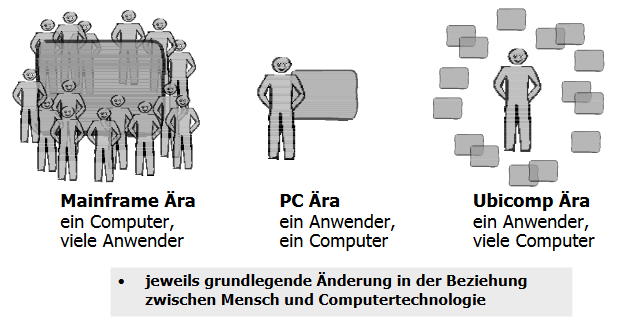
\includegraphics[height = 5cm]{Trend.png}
 \end{center}
 \subsection{Reality - Virtuality Continuum}
 \begin{itemize}
 	\item \textbf{Reality:} Die rohe, reale Welt
 	\item \textbf{Augmented Reality:} Physische Objekte werden erweitert (Infoleiste, Audiokommentar)
 	\item \textbf{Augmented Virtuality:} Die Daten liegen im Fokus und werden durch physische Objekte (Mensch) erläutert (Wetterbericht) 
 	\item \textbf{Virtuality:} reine Information. ``\textit{Alles, was bei Technikausfall nicht mehr da wäre}''
 \end{itemize}
\subsubsection{Virtual Reality vs. Embodied Reality}
Bei \textbf{VR} wird die Realität im Computer integriert, eine neue Realität wird kreiert. \\
Bei \textbf{ER} hingegen wird der Rechner in die Realität integriert, die existierende Realität wird erweitert (Weisers Vision).

\subsection{ParcTab System}
Das ParcTab Ubiquitous Computing Experiment wurde entwickelt um ein UbiComp \textbf{Testbed} zu realisieren. 
\begin{itemize}
	\item[\textbf{Geräte:}] Entwicklung exemplarischer mobiler Geräte. Diese waren nicht persönlich, konnten von allen genutzt werden: \textbf{ParcTab}, \textbf{ParcPad}, \textbf{LiveBoard}, äquivalent zu heutigen \textbf{iPod}, \textbf{iPad}, interaktives \textbf{Whiteboard}
	\item[\textbf{Netzwerke:}] Infrastruktur, um den Informationsaustausch zwischen vielen mobilen Geräten zu gewährleisten.
	\item[\textbf{Kontext:}] Kontext ird genutzt, um die Funktionalität der Geräte und der Interaktion zu verbessern.
	\item[\textbf{Interaktion:}] Entwicklung nicht expliziter Interaktionsmuster.
	\item[\textbf{Applikation:}] Ausnutzung von Lokalität und Kontext.
\end{itemize}

\newpage
\section{``xy''-Computing}
Alles, was hier besprochen wird, endet mit ``Computing''.

\subsection{Mobile Computing}
Erste mobile Computer waren Geräte, die leistungsfähig sind und gleichzeitig gut fürs Büro gebraucht werden können (PDA Phones).
\subsubsection{Smartphones}
Smartphones gehören zu den am meisten verbreiteten Geräten. Diese haben jedoch ihre Vor- un Nachteile:
\begin{itemize}
	\item[\textbf{+}] Ein Gerät, was vieles kann (Schweizer Taschenmesser)
	\item[\textbf{+}] Komfortable Eingabe
	\item[\textbf{+}] Integrierte Dienste
	\item[\textbf{-}] Simpel, jedoch schwer zu entwickeln
	\item[\textbf{-}] Weniger ergonomisch als spezialisierte Geräte
	\item[\textbf{-}] Viruse und Trojaner
\end{itemize}  
\textbf{Prototyp:} Ultra Portable Mobile Computer (Sony Vaio UX)

\subsection{Pervasive Computing}
pervasive (engl.) = penetrativ, allgegenwärtig,\\
 ``\textit{Existiert in jedem Teil von Etwas}''\\
  
IBM haben als erstes UbiComp aus einer Geschäftsperspektive betrachtet. Man wolle nicht einzelne IoT Geräte verkaufen, sondern eine \textbf{Dienstleistung} in Form einer \textbf{Middleware Infrastruktur}. Dieser Service soll dabei auf jedem Gerät laufen, Prozesse beschleunigen (Kauf von Flugtickets, Online Banking) und allen ``das Leben besser machen''. Die Middleware wurde an die verkauft, die diese Middleware nutzen, um ihre eigenen Dienstleistungen zu verkaufen.\\

Hierbei werden die Extrakosten auf den Kunden ausgelagert. Der Kunde zahlt mehr, um eine pervasive Dienstleistung zu bekommen, um die er gar nicht herumkommt.\\
\\
``\textit{Pervasive Computing ist also ein wirtschaftsgetriebener Versuch, die Ideen von Mark Weiser in \underline{monetäre Prozessketten} zu überführen.}''

\subsection{Embedded Computing}
Unter Embedded Computing versteht man die Integration von Sensorik und Aktorik in Alltagsgeräte. Die Recheneinheiten sind dabei sehr günstig, nehmen wenig Platz ein und verfügen über spezielle CPUs. Sie laufen auf bestimmten (echtzeitfähigen) Betriebssystemen, wie \textbf{T-Engine} oder \textbf{ITRON OS}.\\

Weit verbreitete Mikroplattformen für Jedermann (:frau,:divers) sind Raspberry PI und Arduino Mikrocontroller.

\subsection{Wearable Computing}
Hierbei geht es um Rechner, die am Körper getragen werden, ohne das der Nutzer merkt dass er sie trägt. Sie bilden eine Art \textbf{digitale Prothese}, die unsere Fähigkeiten erweitern sollen.\\
\textbf{Beispiele:} Laufschuhe in der Reha, Roulette Shoe, Sonnenbrillen mit MP3
\subsubsection{Exkurs: Cyborg}
Ein Cyborg (\textbf{Cyberkinetic Organism}) ist ein Organismus der aus einem Verbund von organischer und elektronischer Materie besteht. Die (vitalen) Funktionen des Körpers werden dabei elektronisch überarbeitet oder unterstützt. \\
$\implies$ Ist ein Mensch mit Herzschrittmacher schon ein Cyborg?
\subsubsection{Mobilität vs. Engebettheit}
\begin{itemize}
	\item wenig mobil, wenig eingebettet: \textbf{Mainframe}, Traditionelle Business PCs 
	\item wenig mobil, hoch eingebettet: \textbf{Dienste}, sie überall da sind, \textbf{Perv. Comp. } 
	\item hoch mobil, wenig eingebettet: \textbf{Geräte}, die man trägt, \textbf{Mob. Comp.}
	\item hoch mobil, hoch eingebettet: \textbf{Ubiquitous}
\end{itemize}

\subsection{Ubiquitpus Computing}
UbiComp erweitert das Mobile Computing um \textbf{Kontextadaptivität}, \textbf{Datenschutz} und \textbf{Smart Spaces}. Für UbiComp verspricht Feingranularität, die Möglichkeit, viele Probleme zu beobachten und einen großen Schritt in Richtung Effizienz.\\

Jedoch scheitert UbiComp bis dato an vielen Schwierigkeiten in der Umsetzung. Systeme sind \textbf{technisch} komplex, skalieren schlecht, und die meisten verwendeten Netzstrukturen sind heterogen. Es gibt keine einheitliche Norm zur Inter-Gerät-Kommunikation. Hinzu kommen die Probleme in der \textbf{Struktur}: Das Weltmodell ist limitiert (Diskrepanz zwischen Modell und Realität), und die Datenmengen sind enorm hoch.

\subsection{Invisible Computing}
``\textit{Information Appliance}'' \textbf{- Donald E. Norman}\\

Jedem Gerät soll dabei eine einzige Funktionalität zugewiesen werden; Es ist spezialisiert in Information (?).\\
Beispiel Smartphone: Hier herrscht die massenhafte Verfügbarkeit aller Möglichkeiten. Das Menü ist überfordernd. \\
\\
Man möchte lieber eine einzelne Funktion pro Gerät haben. Dadurch verlagert man jedoch das Problem in die nächste Ebene. Statt einem Gerät hat man nun mehrere (\textbf{administrativer Aufwand})!\\
ABER: Erster Schritt in Richtung \textbf{User-Centered-Design}! Erst den den Nutzer verstehen, dann das product entwerfen, und als allerletztes kommt die technische Entwicklung!

\subsection{Calm Computing}
``\textit{Es stellt sich die Frage, was das Ambiente als Produkt ist. Es ist wohl die live passierende Kommunikation. Eine ambiente Umgebung muss demnach aus vielen Produkten bestehen, aber die meisten Geräte sind in sich geschlossen und nicht kompatibel.}'' - Schrader?\\

Bei \textbf{Calm Technology} wechselt das Gerät von der \textbf{Peripherie} in das Zentrum der \textbf{Aufmerksamkeit}. Es ist für den Nutzer also unsichtbar, außer für den Moment, an dem man es bracht. Beispiele sind:
\begin{itemize}
	\item Sauerstoffsensoren
	\item Warnsystem in Autos
	\item \textbf{Dangling String} (Strang, der je nach Auslastung des Netzwerk mehr oder weniger wackelt)
	\item \textbf{Pinwheels}
\end{itemize}
``Technology can communicate, but it doesn't need to speek'' \textbf{- Amber Case}

\subsection{Disappearing Computing}
Disappearnig Computing verfolgt zwei Ansätze:
\begin{enumerate}
	\item \textbf{Physikalisches Verschwinden:} Das Gerät ist so klein / gut integriert, dass man es nicht sehen kann
	\item \textbf{Mentales Verschwinden:} Die Technologie des Geräts rückt in den Hintergrund
\end{enumerate}
Dies ist die Europäische Initiative zu Thema Ambient Computing, die sich längst aufgelöst hat.
\subsection{Organic Computing}
Hierbei werden biologische Prinzipien wie \textbf{Self-CHOP} (Configurating, Healing, Optimizing, Protecting)  und Schwarmtheorie als Grundlage für die Entwicklung der Rechensysteme genutzt. 

\newpage
\section{Miniaturisierung}
Durch den Fortschritt der Technik wurde es möglich, immer kleinere und sogar neue Formen für Geräte zu entwickeln, die für Mensch-Computer-Interaktion genutzt werden können.
\subsection{Moore'sches Gesetz}
Das \textbf{Postulat} von \textbf{Dr. Gordern E. Moore} aus dem Jahr 1968 prophezeit eine \textbf{Verdopplung} der Anzahl an Komponenten auf einem Chip alle 18 bis 24 Monate.\\

Das Postulat hielt bis dato an, aber nur weil auch Chips und Schaltungen kleiner wurden, wodurch auf einen Chip nun mehrere Kerne passten.\\

Es gibt zwar immer bessere und immer kleiner Rechner, jedoch werden die Anwendungen immer komplexer. \textbf{Es gibt einen Fortschritt in der technologischen Entwicklung, aber nicht in der Nutzung der Technik.}

\subsection{Sensorknoten}
Sensorknoten sind kleine, zum Teil münzgroße PCs mit hoher Leistung. Sie werden für das Messen und Sammeln von Daten verwendet. Hier gibt es jedoch Einschränkung bezüglich Batterielaufzeit und Kommunikation. Auch das fehlende User Interface macht die Bedienung umso schwerer.\\
\textbf{Beispiel:} Smarte PostIts, also SmartIts\\

\textbf{Was ist eine sinnvolle Anwendung für solch kleine Rechner?}

\subsection{Smart Dust}
Smart Dust (2001) besteht aus einer Menge von Sensorknoten, wobei ein Knoten gerade mal 1 Kubikmillimeter groß ist. Ein einziger Knoten kann dabei nur sehr simple Operationen durchführen; die komplexe Funktionalität erfolgt in einem dynamischen Sensornetzwerks. Anwendungsfelder sind
\begin{itemize}
	\item Umweltüberwachung
	\item Medizinwissenschaften
	\item Militär
	\item Security usw.
\end{itemize} 

\subsection{Speicherkapazität}
Durch bessere und feinere Technik erhöht sich auch die Speicherdichte. Die Größe der Speichermedien nimmt linear ab, während die Kapazität exponentiell anwächst. Die Kosten sinken logarithmisch. Jedoch sind \textbf{Zugriffszeiten} weiterhin ein Problem.

\subsection{Singularität}
Ausgehend von der derzeit stürmischen Entwicklung der Computertechnik kommt der Roboterexperte Hans Moravec zu der Schlussfolgerung, dass innerhalb der nächsten 40 Jahre Computer die Leistungsfähigkeiten des Menschen allseitig überflügeln werden und als Kinder der Menschheit die Weiterführung der Evolution übernehmen werden.\\

Für Maschinen ist Rechnen viel leichter als Denken und Denken ist viel leichter als Wahrnehmen oder Handeln. Diese Schwierigkeitsabstufung kehrt sich beim Menschen um -- ein Resultat Milliarden Jahre langer Evolution, während der Wahrnehmen und Handeln das Wichtigste war, um weiterleben zu können. Denken und Rechnen wurde erst seit Millionen bzw. seit 10000 Jahren wichtig. Heutige Rechner sind dem Menschen nur dort unterlegen, wo es auf \textbf{Alltagserfahrung} ankommt, den Rechnern fehlt eine Datenbank für Alltagserfahrungen. Bis zum Jahre 1995 erreichten autonome Roboter die Leistungsfähigkeit und das Intelligenzniveau von Insekten, das für einfache Verhaltenssteuerungen ausreicht. Eine Operationsgeschwindigkeit von etwa 10 MIPS und eine Speicherkapazität von 64 MB waren dafür ausreichend bei Kosten von 25000\$ pro Roboter.\\

siehe: \textbf{Hans Moravec}, \textbf{Ray Kurzweil}

\subsection{Gefahren des exponentiellen Wachstums in der Wirtschaft}
Das kapitalistische System ist auf Wachstum fokussiert. Will man ein exponentielles Wachstum an Erzeugnissen (Output) erreichen, so muss in Folge dessen auch der Zufluss an Ressourcen exponentiell steigen. Werden die Ressourcen knapper, kommt es zu einem Crash des ökonomischen Systems. 
\begin{center}
	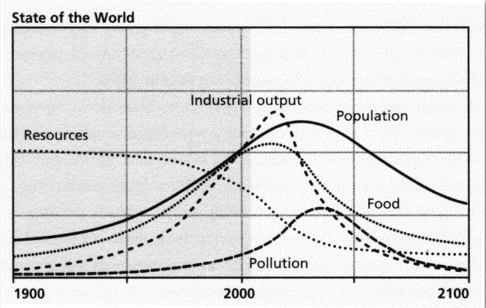
\includegraphics[height = 4cm]{growth.png}
\end{center}
 Prognosen über die Entwicklung der Zukunft aus dem status quo der Wachstumsentwicklung können leider nur schwer gemacht werden. Es kann sein, dass man in der Entwicklung auf eine ``Schallmauer'' (Concorde Flieger) trifft, ab der eine weitere exponentielle Entwicklung nicht mehr wünschenswert ist.
 \subsection{Nanoroboter}
 Nanoroboter sind nanogroße ($<1$mm) smarte Geräte die Computing, Sensing und Actuation durchführen. Sie werden zum Aufbau medizinischer Nanonetzwerke verwendet, um Krebs, Entzündungen und die Entwicklung allgemeiner Krankheiten zu überwachen.\\
 \\
 
 Dabei müssen viele komplexe mathematische Probleme gelöst werden, und es stellt sich die Frage, ob dies mit so kleinen Rechnern überhaupt möglich ist. Hierfür werden Nanogeräte in \textbf{Komplexitätsklassen} eingeordnet, um eine Aussage darüber zu treffen, was dieses Gerät kann und was es nicht kann.
 \begin{itemize}
 	\item[\textsc{AC}$^0$:] Addieren, Subtrahieren, Signum
 	\item[\textsc{NC}$^1$:] Multiplikation, Division, Parität
 	\item[\textsc{L}:] Logarithmus, Reach (\textbf{Netzwerkfähigkeit!})
 \end{itemize}
Dies impliziert, dass nicht jeder Algorithmus auf Nanobots übertragen werden kann. Es gibt also nicht ``plenty of room at the bottom''.
\newpage

\section{Wearable Computing}
Wearable Computing sind Rechner, die am (menschlichen) Körper getragen werden. Sie sollen mobile Nutzer \textbf{unterstützen} (Guides, Übersetzer, Reparatur), Körperfunktionen \textbf{ersetzen} (Prothesen, Implantate) oder die körperlichen Funktionen \textbf{erweitern} (Speicher, Funktionalität).\\

Beispiele:
\begin{itemize}
	\item \textbf{Smarte Schuhe:} Tracken Schrittanzahl, automatisches Zubinden
	\item \textbf{Head Mounted Displays:}  Smart Glasses, Remembrance Agent (kontext-relevante Informationen abhängig von Ort und Nutzer)
	\item \textbf{Smarte Socken:} Identifiziert falsche Laufbewegungen
	\item \textbf{Smarte Juwelierwaren:} Mikrofone und Lautsprecher in Ringen und Ketten integriert. Speichermedium in Manschettenknöpfen.
	\item \textbf{Smart Watches:} Ökosystem von smarten Geräten
\end{itemize}
\subsection{Formfaktoren}
Die Platzierung und der komfort von tragbaren Geräten spielt eine große Rolle in Bezug auf \textbf{Nutzerfreundlichkeit}, \textbf{Interaktion} und mögliche \textbf{Nutzungsszenarien}. Die Entwicklung solcher Geräte entsteht für Stellen am Körper, die bei jedem Mensch relativ gleich groß sind und \textbf{geringe Flexibilität} benötigen (Nacken, Fuß, Schienbein).
\subsection{Herausforderungen}
\begin{enumerate}
	\item \textbf{Konnektivität:} Man möchte eine nahtlose Konnektivität über mehrere verschieden Arten von Netzwerken erreichen. Dazu gehört auch \textbf{gelegentliche} Verbindung (abhängig von der Lokalität) und die \textbf{lokale Kommunikation}.
	\item \textbf{Nutzerfreundlichkeit:} Verschiedene Methoden der Interaktion (visuell und auditiv) sowie deren Belastung auf die Sinne (medizinische Sicherheit) müssen berücksichtigt werden. Zudem müssen die Geräte sozial akzeptabel sein.
	\item \textbf{Situiertheit:} Auffangen und Interpretieren von Kontextinformationen, welche zur \textbf{persönlichen Assistenz} (Augmentation) genutzt wird.
\end{enumerate}

\newpage
\section{Smart Clothes}

\newpage
\section{Energy Harvesting}
Obwohl ein exponentielles Wachstum bezüglich Komponentenanzahl/Schaltkreisdichte auf Chips und Speicherdichte seit Jahren beobachtet werden kann, so trifft das\textbf{ Moore'sche Gesetz} leider nicht auf die Entwicklung der Batterien zu. Diese haben sich in den letzten 10 Jahren nur um $20\%$ verbessert, das Wachstum ist linear. Dies liegt daran, dass Physik nicht Technologie ist, und man da recht schnell auf seine ``Schallmauer'' trifft.\\

\textbf{Energie} wird beschrieben durch Joule ($kg\cdot m^2 / sec^2$).\\
\textbf{Leistung} wird beschrieben durch Watt ($kg\cdot m^2 / sec^3 = J / s$) \\
$100$ Kcal/h entspricht dabei 115 Watt
\begin{center}
	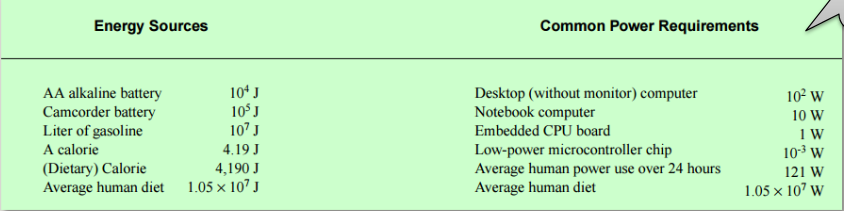
\includegraphics[height = 3cm]{Energy.png}
\end{center}

\subsection{Koomey'sches Gesetz}
Das Pendant zum Moore'schen Gesetz. Dieses Gesetz besagt, dass die Menge der Batteriekapazität die für eine Anzahl von Berechnungen verbraucht wird, sich alle 18 Monate halbiert.

\subsection{Jevon's Paradoxon (Rebound Effekt)}
Es ist eine naive Annahme zu glauben, dass durch die steigende Effizienz der Technik die für den Menschen gebrauchten Ressourcen länger reichen. Denn: Sobald etwas energieeffizienter ist, wird es günstiger. Dadurch wollen es mehr Leute haben, da sie es sich nun leisten können.\\

Nach dem Paradoxon wird der Verbrauch mit steigender Effizienz nicht sinken, sondern er wird sich erhöhen. \\
\textbf{Die Verbreitung wird größer, als der Effizienzvorteil.}

\subsection{Das Energie-Problem}
\begin{itemize}
	\item \textbf{Etwa $40\%$ der Energie wird im Standby-Modus ungenutzt verbraten.}\\
	\textbf{Beispiel:} Googles Serverfarmen benötigen mehr Energie für die Kühlung, als für die Berechnungen. Man kann nun die Serverfarmen da aufstellen, wo es kalt ist (\textbf{Ambiente ausnutzen}) oder da, wo die Abwärme gebraucht wird (\textbf{dem Ambiente dienen}). Das ist aber Energy \textbf{Avoidance}, nicht Energy \textbf{Harvesting}! Besser wäre, mehr nachhaltige Energiequellen zu nutzen (Wasserturbinen, Solar)\newpage
	\item \textbf{IoT benötigt Batterien, aber sie sind schlecht!}\\ Es werden mehr in den Verkehr gebracht, als wieder eingesammelt. Manche Geräte lassen sich mit Solarenergie oder Dynamo betreiben. \\
	\textbf{Beispiele:} Self-Powered Image Sensors, Backscattering von elektromagnetischen Wellen
	\item \textbf{Wie deckt man den Energiebedarf von sehr kleinen Geräten?}\\
	Gerätegröße skaliert nicht mit benötigter Energie / Batteriegröße.\\
	\textbf{Beispiel:} Smart Dust werden durch passive optische Kommunikation aufgeladen. (\textbf{Corner-Cube-Retroflector}). Woher kommt die Energie für aktive Kommunikation?
\end{itemize}
\subsection{Mögliche Lösungen}
\begin{center}
	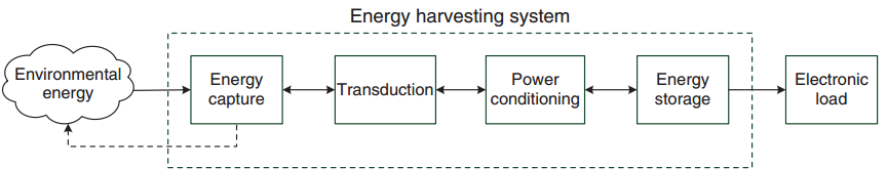
\includegraphics[height = 2.5cm]{Harvesting.png}
\end{center}

Mögliche Lösungen für die Energieprobleme sind \textbf{Micro Energy Harvesting}, das Ausnutzen von \textbf{physische Quellen} (Piezo, Pyro, Thermoelektrik, Induktion) oder \textbf{biologische Quellen} (Vibrationen, Abwärme, Sprache, Herzschlag).
\subsubsection{Mensch als Quelle}
\begin{itemize}
	\item Druckplatten im Boden (pavegen)
	\item Fahrräder
	\item Self-Powered Tastaturen
	\item Thermoelektrische Wearables
\end{itemize}

\newpage
\section{Neue Materialien und Formen}
Flexible Materialien erlauben eine komplett neue Art von smarten Objekten.
\begin{itemize}
	\item Fiberoptik
	\item flexible Substrate
	\item Organic Displays
\end{itemize}
Doch wie bauen wir diese Sensoren und Aktoren in Kleidung ein? Das führt zu Problemen beim Waschgang, neuen Müllbergen... \\
$\implies$ \textbf{Der Umwelteffekt ist grauenhaft!}
\subsection{Electronische Tinte / Papier}
\begin{itemize}
	\item \textbf{Gyricon:} Schwarz-Weiße Bälle zwischen zwei Platten. Durch statische Aufladung kam entweder die weiße oder die schwarze Seite nach oben.
	\item \textbf{E-Ink:} Nachfolger von Gyricon. War schneller, dünner und präziser.
	\item \textbf{OLED:} Biegbare Panels aus LEDs
\end{itemize}
Solche Displays waren nun überall einbaubar: \textbf{Schneidebrett}, \textbf{Maßband}, \textbf{Snowboard} etc.\\
\textbf{ Jedoch ist eine Nachahmung des original analogen als ambiente Technologie nicht immer empfehlenswert}, siehe zB Digital Newspaper.

\subsection{Neue Formen}
Durch neue Art der Produktionstechnik ist es möglich, Objekte in neuen Formen zu erstellen.\\
Dank beispielsweise \textbf{3D-Druckern} kann man alles produzieren lassen, was man möchte.\\

Jedoch ist die Einrichtung der Maschine teurer und schwerer, als der Druck selbst! \textbf{Eine Einzelteilentwicklung ist somit überaus kostenintensiv}.

\subsection{Konvergenz von Funktionen}
Idee dahinter ist ein Verbund von Funktionen, also der Einbau von Geräten in existierende Geräte. \textbf{Hardware} kann durch weitere Hardware erweitert werden, was eventuell zu mehr Kosten und Inkompatibilität mit anderen Geräten führt.\\
\\
Alternativ kann man Geräte entwickeln, dessen Verbund eine neue, verbesserte Funktionalität ermöglicht.(4 gleiche Displays $\implies$ 1 großer Bildschirm)  

\subsection{Modulares Design}
PHONEBLOCKS ist eine Open Source hardware Plattform, die ein Handy anbieten wollte, welches in seinen Komponenten komplett modular ist. Batterien, Kameras, Specher etc können somit schnell und einfach ausgetauscht werden. Der Trend ging in die Richtung, \textbf{Hardware so gestaltbar wie Software} zu machen. \\

Es gab viele Probleme, vor allem fehlende Robustheit der Verbindungsstücke einzelner Module führte zum scheitern des Projekts.

\subsection{Displays}
Flexible und faltbare Displays erlauben es, neue formändernde Objekte zu kreieren. Dadurch können Displays auf jede mögliche Oberfläche platziert werden. 

\newpage
\section{Wearables}
\newpage
\section{Smarte Kleidung}
\newpage
\section{Kontektbewusstsein}
\subsection{Was ist Kontext?}
Man versucht zu begreifen, was man \textbf{sinnvolles} mit Sensoren und Aktoren machen kann. \textbf{Kontext} ist dabei etwas mit gewissem Muster/Struktur/Beschaffenheit, welches Deutbarkeit erzeugt. Kontext abstrahiert das, was uns umgibt. Wir möchten die Information der Umgebung festhalten um damit sinnvolle intelligente Entscheidungen zu treffen.\\

\textbf{Kontext ist jede Information, die genutzt werden kann, um die Situation einer Entität zu charakterisieren. Eine Entität kann dabei eine Person, Ort oder Objekt sein, welche für die Person-Applicatino-Interaktion relevant ist.}\\

``\textit{Who, What, Where, When and Why}'' \\

Für Sensoren in kontext-bewussten Umgebungen besteht dabei die Schwierigkeiten, diesen zu sehen. Prädiktion und Intention des Nutzers sind keine Quantitäten, die irgendwie physikalisch messbar sind. \\

``\textit{Es gibt Sensoren für What, aber nicht für How}''

\subsection{Kontextbewusstsein}
Ein System zählt als \textbf{kontext-bewusst}, wenn es Kontext benutzt, um Informationen und Dienste dem Nutzer bereitzustellen, wo die Relevenz vom Nutzer abhängt. Dabei geht es um korrekte
\begin{itemize}
	\item \textbf{Präsentation:} Relevante Informationen werden dem Nutzer gezeigt
	\item \textbf{Ausführung:} Richtige Services starten in bestimmten Situationen
	\item \textbf{Bedeutung:} Kontextdaten werden Sensordaten hinzugefügt
	\item \textbf{Empfehlung:} Nutzer bekommen Tipps zu zukünftigen Aktionen
\end{itemize}

\subsection{Kontextmodellierung und Anschaffung}
\begin{enumerate}
	\item \textbf{Entität} wird observiert von Kamera, Mikrofon, Biosensoren, woraus man dann
	\item \textbf{Daten} erhält, zum Beispiel Druck, Feuchtigkeit, Beleuchtung, Position etc. Durch Interpretation der Daten bildet sich
	\item \textbf{Kontext} zu einem Ort, einer Identität, einer Aktivität, oder gar Emotion. als letztes benötigen wir eine
	\item \textbf{Repräsentation} des Kontext, zB als Key-Value, Markup Scheme, Graphische Darstellung usw.
\end{enumerate}
\subsection{Sensortypen}
Man unterscheidet in {physikalische} und {virtuelle} Sensoren.\\

\textbf{Physikalische Sensoren} messen physikalische Quantitäten und wandeln diese in ein Signal um.\\
\textbf{Virtuelle Sensoren} führen indirekte Messungen abstrakter Daten durch. Es ist ein Verbund aus real gemessenen Quantitäten und einem Modell, anhand dessen eine Zielgröße berechnet wird.\\

Messen / Wahrnehmung ist die Grundlage der Kontextinformation. Viele Low-Level Sensoren (Sensortypen unendlich viele vorhanden!) führen \textbf{Messungen} durch und bereiten die Daten auf (\textbf{Preprocessing}). Danach werden \textbf{Features} extrahiert (Kontext ``Atome'') und anhand der Features wird klassifiziert (Bayes'sche \textbf{Klassifikation}). So oder so ähnlich.\\

\textbf{Gierad Laput} entwickelt einen Supersensor, der viele verschiedene Low-Level Sensoren beinhaltet. \\

\begin{center}
	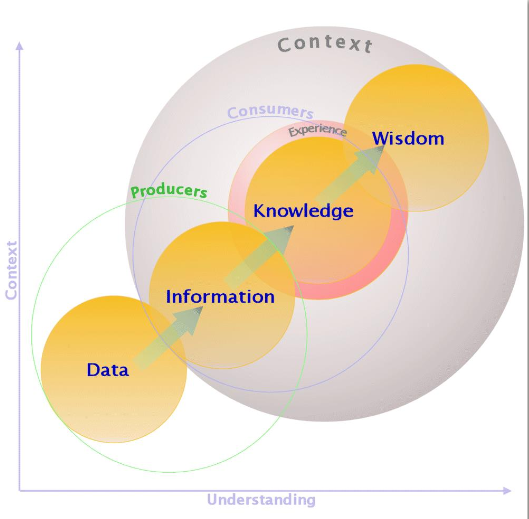
\includegraphics[height = 8cm]{Kontext.png}
\end{center}
\newpage

\section{Kontext-Bewusste Software Architekturen}
Für die Softwarearchitektur werden garantiert \textbf{Sensorik}, \textbf{Aktorik} und viel \textbf{Machine Learning} benötigt. Ein eingeschränktes Testlabor für solche Systeme gibt es leider nicht.\\

\textbf{Der Test eines solchen Systems kann nur in der realen Umgebung erfolgen.}
\subsection{Frameworks und Toolkits}
\subsubsection{Widget-basierte Systeme}
Widget ist einfach ein schickeres Wort für Treiber oder Controller, wobei die \textbf{Businesslogik} und Komplexität ser Sensoren hinter einer \textbf{GUI} versteckt werden.
\subsubsection{Blackboard-basierte Systeme}
Das Blackboard ist das Tuple Space eines Systems. Hierbei holen sich Apps Informationen von einem persistenten Speicher, sie wissen nichts von den Sensoren, die Sensoren selber nur den Speicher füttern.
\subsubsection{Was ist nun besser?}
Widgets sind zu \textbf{rigide}, und jeder Sensor kann mehrere passende Widgets haben (\textbf{Überblick}?). Bei Entwicklung eines neuen Widgets muss die \textbf{API ebenfalls neu entwickelt} werden. \\
Blackboards hingegen sind ineffizient hinsichtlich des Speicherns und der Suche der Daten. Es kann dadurch vermehrt zu Synchronisationsproblemen kommen.
\subsection{Ambient DynamiX}
Idee: Kombination von Widgets und Blackboards. DynamiX läuft als Android (da iOS aus Sicherheitsgründen keine Thread-Kommunikation erlaubt) Background Service. Als Nutzer verwaltet man die damit verbundenen Apps, Zugriffe, PlugIns etc.

\subsection{Ambient Web}
AmbiWeb ist eine browserbasierte Version von Ambient DynamiX. Dadurch hat man zwar eine plattformübergreifende Version geschaffen, der Zugriff auf die Handyhardware gelingt jedoch nur mithilfe von weiteren Browser PlugIns, für die die zukünftige Android-Unterstützung nicht ganz klar ist.\\

\textbf{Ziel: In eine Umgebung reinkommen, NFC Tag scannen, AppServer zeigt Content, nach Bestätigung werden benötigte Module aus dem PlugIn-Repository heruntergeladen, und der Raum kann nun in vollen Zügen genutzt werden.}

\newpage
\section{Identifikation}
\subsection{Entität, Identität?}
Eine \textbf{Entität} ist eine distinkte, reale Existenz. Es ist eine individuelle Einheit, die nicht unbedingt ein physische Form haben muss.\\
Eine \textbf{Identität} ist die Differenz oder Charakter eines Individuum, welches ihn von seinen Genossen gleicher Art trennt. Jeder hat seine eigene Identität.\\
Die \textbf{Ähnlichkeit} wird an einem \textbf{Attribut} bestimmt, welches als \textbf{Vergleichsmetrik} dient.\\
\\
\textbf{Wie misst man eine Identität?}\\

Eine Identität wird in der Regel \textbf{nie überprüft}, sondern es werden Attribute mit einem anderen Objekt verglichen (Personalausweis mit Urkunde oder Datenbank).
\subsection{Objekt, Subjekt?}
Ein \textbf{Objekt} kann durch ein anderes System identifiziert werden (Kamera, Barcode) und es kann Identifikations-Mechanismen bereitstellen (\textbf{aktive Reflektion} auf das System durch RFID, Bluetooth).\\
Ein \textbf{Subjekt} kann identifiziert werden und auch sich selber identifizieren (ID, DNA, Fingerabdrücke).

\subsection{Identifikations-Technologien}
\begin{itemize}
	\item Barcodes
	\item RFID
	\item Visuelle Erkennung von Form, Farbe, Struktur
	\item Akustik: Stimme
	\item Biometrisch durch Fingerabdrücke und Retina
\end{itemize}
Es is jedoch zu beachten, dass eine \textbf{Korrelation zwischen ID-Technologie und Identität nicht unbedingt vorhanden ist}.
\subsubsection{Visual Microphone}
Idee: Jedes leicht verformbare Objekt könnte als Mikrofon genutzt werden. Schalldruckwellen erzeugen ein \textbf{bestimmtes Muster} an leichten Objektstrukturen, wie \textbf{Chipstüten} oder Pflanzen.
\subsubsection{Radio Frequency IDentification}
Zusammenspiel von Transponder und Reader wird als Identifikationsmaßnahme genutzt.
Der \textbf{Transponder} ist dabei ein Objekt, welches identifiziert werden muss. Es beinhaltet einen Mikrochip, Speicher und eine Koppelelement.\\
Der \textbf{Reader} hingegen sendet und erhält modulierte Signale. Dafer enthält er selbstverständlich die benötigten Module.\\

RFID funktioniert dabei auf zwei verschiedenen Weisen:
\begin{itemize}
	\item \textbf{Induktives Koppeln:} Der Emitter (Reader) hat eine große stromdurchflossene Spule, durch die eine Spannung induziert wird. Der Chip hat ebenfalls eine (kleine) Spule in Parallelschaltung mit einem Kondensator. Die Resonante Schaltung entzieht dem Magnetfeld Energie, welche vom Reader gemessen wird.
	\item \textbf{Backscatter Coupling:} Elektromagnetische Welle wird am Transponder reflektiert, wenn die Resonanzfrequenzen (13MHz) stimmen. Der Transponder entzieht dabei Informationen aus dem Signal, die dann vom Reader gelesen werden.
\end{itemize}

\subsubsection{Transpondertypen}
Transponder gibt es in jeglicher Form. \textbf{Aktive} Transponder unterscheiden sich dadurch, dass sie eine eigene Batterie haben und somit über längere Distanz kommunizieren können. \textbf{Passive} Transponder werden öfter verwendet, da sie keine extra Batterie brauchen. Sie ``ernähren'' sich vom elektromagnetischen Feld, was der Reader aussendet.

\subsection{Wozu?}
RFIDs können überall verwendet werden, wo eine schnelle Identifikation vorteilhaft sein kann. Krankenhäuser, Mautstationen, Bibliotheken etc.\\

Man möchte dadurch das \textbf{Datashadow}, eine Lücke zwischen physikalischen Zustand und medialer Repräsentation, schließen. Dies wäre auch ein weiterer Schritt in Richtung \textbf{Industrie 4.0} (Vollautomatisierung von Herstellungsprozessen, objektgetriebene statt systemgetriebene Fabrikation)

\newpage
\section{Ambiente Interaktion}
Man möchte \textbf{Natural User Interfaces (NUI)} entwickeln, um eine möglichst intuitive Mensch-Computer-Interaktion zu gewährleisten.\\
Es gibt eine \textbf{digitale Kluft} zwischen Realität und Virtualität. Menschen sind keine Cyberwesen. \textbf{Avatare} hingegen schon; es ist das virtuelle Dasein des Menschen im Cyberspace, welches aber keine menschlichen Fähigkeiten besitzt. Man benötigt also ein Interface, um \textbf{Tangibles} (=tragbare Geräte) und digitale Daten/\textbf{Informationen} zu verbinden.

\subsection{Touch Interfaces}
Die ersten Touch Interfaces gibt es seit dem in 2006 von Jeff Han entwickelten ``\textbf{Multi-Touch}''. Dabei wurden zwischen zwei Platten Lichtstrahlen ausgesendet: Die Berührung der Platte sorgte für eine Streuung des Licht, die detektiert werden konnte.

\subsection{Tangible Media (TUI)}
Hierbei möchte man sich von der GUI trennen (die \textbf{Line of Sight} und wenig menschliches Können erfordert) und einen Schritt in Richtung \textbf{physische Interaktion} machen. Man möchte also physische Objekte bewegen oder drehen, um eine Interaktion auf den Daten auszuführen. \\

``\textit{Im Grunde ist Tangible Media \underline{begreifbare Interaktion}.}''\\

Bei Tangible Media wird die Welt selbst zum Interface, man \textbf{erweitert} existierende physikalische Objekte mit digitalen Technologien.
\begin{center}
	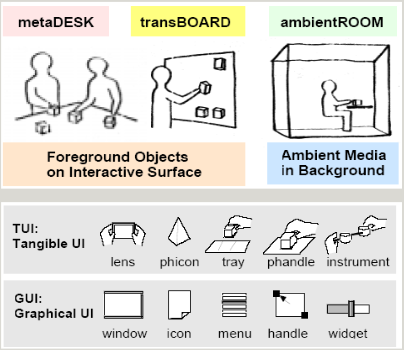
\includegraphics[height = 4cm]{TUI.png}
\end{center}
\begin{itemize}
	\item \textbf{Interaktive Oberflächen:} Transformation der Architektur (Wände, Türen,...) in ein aktives Interface
	\item \textbf{Koppeln von Bits und Atomen:} Nahtloses Koppeln von begreifbaren Objekten
	\item \textbf{Ambiente Medien:} Nutzung von Sound, Licht, Luft, Wasserbewegung...
\end{itemize}
\subsection{Ambient Awareness}
Bei Ambient Awareness werden physische Geräte ausgenutzt, um Informationen \textbf{subtil} anzuzeigen (Dangling String, Pinwheel Project). Zum Verständnis dieser Informationen wird jedoch \textbf{Kontext} benötigt.
\subsection{TUI Projekte}
\begin{itemize}
	\item \textbf{Music Bottles:} Information in Form von Sound ist in einer Flasche vorhanden. Das Öffnen/Schließen des Mediums (Flaschenkorken) repräsentiert Wiedergabe/Stoppen der Information.
	\item \textbf{reacTable:} Smarter Tisch. Auf die Stoffoberfläche werden unter dem Tisch befindliche Kameras gerichtet, die Objekte identifizieren und Interaktion erlauben. 
	\item \textbf{SandScape:} Ein Sandhaufen in einer Kiste, der zum Design und Verständnis von Landschaften verwendet wird. Durch Modifikation des Sandes können 3D Oberflächen verändert werden. Die Architektur ist jedoch sehr kostspielig (von oben und unten wird projiziert, oben eine Tiefenkamera, Berechnungen der Projektion...)
	\item \textbf{Electrick:} Leitende Sprühfarbe kann überall aufgetragen werden, um jedes Objekt zu einem Touch Interface zu machen (Verkabelung? Präzision?)
\end{itemize}
\subsection{OUI}
\textbf{Organic User Interfaces (OUI)} sind um die Flexibilität erweiterte GUIs. Dabei handelt es sich um \textbf{verformte} Displays, \textbf{flexible} User Interfaces (Eingabe erfolgt durch Verformung) und \textbf{kinetische} User Interfaces (Form wird durch den Rechner bestimmt).

\newpage
\section{Smart Spaces}
\begin{center}
	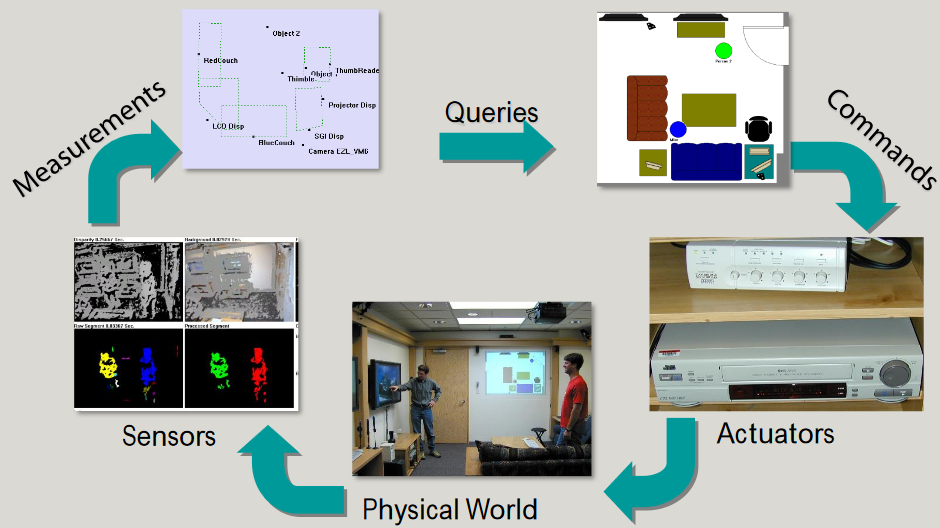
\includegraphics[height = 5cm]{SmartSpace.png}\\
	Easy Living von Microsoft
\end{center}
Ambient Computing wird dazu genutzt, um alltägliche Orte zu \textbf{Smart Spaces} zu bereichern. Bei Smart Spaces geht es jedoch nicht darum, eine zentrale Intelligenz oder eine überliegende KI Instanz zu schaffen, sondern die Aggregation und Kommunikation der Geräte soll intelligent sein.
\subsection{Smart Kitchen}
Smart Kitchen ist ein Beispiel für ein Smart Space. Hierbei werden die Oberflächen und Geräte so erweitert, dass die von ihnen ausgesandte kontextsensitive Information zur Vereinfachung von Prozessen genutzt werden kann.
\begin{itemize}
	\item Rezepte werden auf eine Oberfläche projiziert
	\item Kühlschrank ist transparent, um Inhalt anzuzeigen
	\item beleuchteter, smarter Wasserhahn
\end{itemize}
\subsection{Persuasive Interfaces}
persuasive (engl.) = überzeugend\\

Bei Ambient Persuasion möchte man den Nutzer zu einer \textbf{bestimmten Nutzung} des Geräts verleiten/überzeugen. Das Ambiente (kontextbewusste Geräte) sagt einem, wie man das Gerät benutzt oder was in einer bestimmten Situation zu tun ist.
\subsection{Smart Spaces?}
\subsubsection{Smart Home}
Ein Projekt zur Entwicklung eines vernetzten und mit verschiedener Sensorik und Aktorik ausgestatteten \textbf{bewussten Hauses}.
\subsubsection{Smart Museum}
Siehe HolstenTOUR
\subsubsection{Smart Neighborhood}
\subsubsection{Smart City}
Siehe Smart Santander
\begin{itemize}
	\item Verkehr- und Parkplatzmanagement
	\item Busverkehr Optimierung
	\item Straßenlicht
	\item Müll
	\item Car Sharing
\end{itemize}
Auch Interessant: \textbf{Sound of the City}, \textbf{MeinLübeck}

\newpage
\section{Ethical, Legal and Social Implications}
Neben vielen technischen Herausforderungen (Standardisierung, Nutzerfreundlichkeit, etc.) gobt es auch viele nicht-technische Herausforderungen.
\begin{itemize}
	\item \textbf{Legalität:} Darf das genutzt werden?
	\item \textbf{Datensicherheit:} Ist das System sicher?
	\item \textbf{Finanzierung:} Können wir uns das System leisten?
	\item \textbf{Nachhaltigkeit:} Ruinieren wir unseren Planeten?
	\item \textbf{Ethische/Soziale Konsequenzen:} Können wir human bleiben?
	\item \textbf{Akzeptanz:} Möchten wir das überhaupt?
\end{itemize}

\subsection{Legalität}
Im deutschen Grundgesetz gibt es das Recht auf die körperliche Unversehrtheit (Art. 2). Dieses Gesetz kann jedoch durch andere Gesetzgebungen überschrieben werden (Religion bsp.) und schützt auch nicht das \textbf{soziale Wohlbefinden}.

\subsection{Datensicherheit}
Neben der physischen Sicherheit (Roboterarm der netterweise einen nicht durchbohrt) gibt es auch die persönliche Datensicherheit.\\
Sicherheit wird vor allem anhand von
\begin{itemize}
	\item Vertraulichkeit (Zugriff wird nicht authentifizierten Personen verweigert )
	\item Integrität (Mensch Maschine)
	\item Verfügbarkeit (Dienstleistungen sollen autorisierten Personen nicht verweigert werden)
\end{itemize}
gemessen.

\subsection{Privatsphäre}
``\textit{Sind Smart Spaces das Panoptikum der Zukunft?}''\\

In vielen Ländern gibt es mittlerweile Überwachung öffentlicher Plätze. Das Ziel ist, durch Überwachung die Kriminalität zu reduzieren, was bislang kaum bis gar nicht geklappt hat. \\

Es kommt oft zum \textbf{Monitoring Dilemma}: Man möchte oder muss Menschen bei Ambient Assisted Living beobachten und observieren, um sie zu assistieren. Der Nachteil dabei ist natürlich die \textbf{unerwünschte Überwachung}.\\
Ein anderer Ansatz ist \textbf{Sousveillance}, also die Observierung des Observierenden. Dabei werden Dashcams, mobile Kameras etc verwendet, um Aktionen in der Umgebung zu melden.

\subsection{Privatsphäre in UbiComp}
Sensoren sind überall angebracht, und können alles messen. Durch diesen hohen Grad der Verbreitung und Integrität der Technologie wird \textbf{Invasion} und \textbf{Kontrolle} immer einfacher. \\

Die Gesellschaft spaltet sich in zwei Lager: Die, die auf \textbf{Bequemlichkeit} (Convenience) bestehen, und die, die auf ihre \textbf{Privatsphäre} bestehen.

\subsection{Nachhaltigkeit}
Alles muss irgendwie produziert werden.\\
 \textbf{Wie groß ist der ökologische und soziale Fußabdruck?} (Abbau von Metallen in Kinderarbeit, Elektronikmüllberge) 
 
 \subsection{Soziale Implikationen}
 ``\textit{Unsere ganze Unterhaltungsindustrie ist ein Hilfsmittel, um uns selbst wirkungsvoll zu vergessen}'' \textbf{- Richard David Precht (2010)}\\
 
 \begin{itemize}
 	\item Hohe Nutzung von Smartphones wird mit Verminderung der Intelligenz verbunden. Wissen ist on-demand da, wozu sich alles merken?\\
 	$\implies$ \textbf{Degeneration des Menschen}
 	\item Vermehrte Nutzung von Smart Devices führt zum Verlust der eigenen Autonomie
 \end{itemize}
\subsubsection{Intelligenz vs. Smartness}
\textbf{Intelligenz} ist Verständnis und das Potenzial, Fähigkeiten zu erlernen. Es ist die \textbf{kognitive Power}.\\
\textbf{Smartness} (Schlauheit?) dagegen ist ein Zustand. Es ist das Ergebnis eines \textbf{Lernprozesses} und die Fähigkeit, zu handeln.\\

Smarte Umgebungen bieten viel Rechenpower, verlangen aber auch viel Kontrolle über die Aktionen und sind meist intransparent. Es ist eine \textbf{autonome Assistenz}.\\
Smarten Nutzern hingegen stehen weniger Power und weniger Präzision zur Verfügung, dafür jedoch mehr Kontrolle über die eigene Privatsphäre. Es ist eine \textbf{assistierte Autonomie}.\\

Neu Formen der Technologie ändern das soziale Verhalten des Menschen (Handys bei Konzerten, Smombies). Dabei ist die Nutzung des Smartphones gefährlich in Zusammenhang mit Bewegung des Menschen (Fahren, Hindernisse übersehen).


\end{document}